% For instructions,
\documentclass[reprint, amsmath, amssymb, aps, onecolumn]{revtex4-2}

%\usepackage[norsk]{babel}
%Uncomment this if you want to write in Norwegian

\usepackage{graphicx}% Include figure files
\usepackage{dcolumn}% Align table columns on decimal point
\usepackage{bm}% bold math
\usepackage{hyperref}% add hypertext capabilities
\usepackage{booktabs}
\usepackage{float}
\usepackage{siunitx}
\usepackage{subcaption}
\usepackage{xcolor}
\usepackage{hyperref}
\hypersetup{
    colorlinks=true,
    linkcolor={red!60!black},
    filecolor=magenta,
    urlcolor=cyan,
    citecolor=blue!80!black
}

\usepackage[raggedright]{titlesec}
% \usepackage{minted}

% \renewcommand{\vec}[1]{\mathbf{#1}} %ny definisjon av \vec så det blir bold face i stedet for vector-pil.
\newcommand{\LLRA}{\\[-1.3\baselineskip] $\Longleftrightarrow$ \\[-1.3\baselineskip]}

% \newcommand{\up}{\uparrow}
% \newcommand{\down}{\downarrow}
% \newcommand{\up}{\frac{1}{2}}
% \newcommand{\down}{-\frac{1}{2}}


% \newcommand{\dd}[4]{\left(\frac{\partial #1}{\partial #2}_{#3,#4}\right)
\newcommand{\dd}[3]{\left(\frac{\partial #1}{\partial #2}\right)_{#3}}
\DeclareMathOperator{\tr}{tr}

% \usepackage{braket}
% \usepackage{minted}

\usepackage{polynom}
\begin{document}
\title{FYS4130 - Oblig 2}

\author{Mikkel Metzsch Jensen}
\noaffiliation
\date{\today}
\maketitle
%
\onecolumngrid

\section*{Problem 1}
\noindent We study the 1D "spin" chain of length $L$ with $N$ spins and periodic boundary conditions governed by the hamiltonian
\begin{align*}
  H = -J \sum_{i=0}^{L-1} \delta_{\sigma_i, \sigma_{i+1}}, \qquad J > 0,
\end{align*}
where $\sigma_i$ takes spin values $\{0,1,2\}$. We measure the length in units of lattice spacing such that $N=L$. 
%
%%
%
\subsection*{1a)}
\noindent The canonical partition function $Z$ for a discrete ensemble is given as
\begin{align*}
  Z = \sum_{\{\sigma \}} e^{-\beta H} 
    = \sum_{\{\sigma \}} e^{\beta J \sum_{i=0}^{L-1} \delta_{\sigma_i, \sigma_{i+1}}}, 
\end{align*}
where $\{\sigma\}$ denotes the sum over all possible configurations of the three spin values for the L spin sites. We can rewrite the sum in the exponent as a product and introduce the transfer matrix $T$ as follows.
\begin{align*}
  Z = \sum_{\{\sigma \}} \prod_i^{L-1}  e^{\beta J \delta_{\sigma_i, \sigma_{i+1}}} 
    = \sum_{\{\sigma \}} \prod_i^{L-1} T_{\sigma_i, \sigma_{i+1}}, \qquad   
    T = \begin{pmatrix}
      e^{\beta J} & 1 & 1 \\
      1 & e^{\beta J} & 1 \\
      1 & 1 & e^{\beta J}
    \end{pmatrix}.
\end{align*}
We can write out the product and use the general expression $A^2_{i,j} = \sum_{k} A_{i,k}A_{k,j}$, such that we get
\begin{align*}
  Z = \underbrace{\sum_{\sigma_0=0}^2 \sum_{\sigma_1=0}^2 \cdots \sum_{\sigma_{L-1}=0}^2}_{L} T_{\sigma_0, \sigma_1} T_{\sigma_1, \sigma_2} \cdots T_{\sigma_{L-1}, \sigma_{0}} = \sum_{\sigma_0=0}^2 T_{\sigma_0, \sigma_0}^{L} = \tr(T^L),
\end{align*}
where $\tr(T^L)$ denotes the trace of $T^L$. The next step is to diagonalize $T$ as $T = PDP^{-1}$, where $D$ is the diagonal matrix containing the eigenvalues on the diagonal and $P$ is an invertable matrix where the columns form a basis consisting of eigenvectors of T. Given a diagonalization we can use that the trace is inviariant under similarity transformations (such as the diagonalization) and that the trace of a product of matrices is invariant under cyclic permutation \cite{Svendsen}(P. 429-430)
\begin{align*}
  \tr(T^L) = \tr\underbrace{(PDP^{-1}PDP^{-1}\cdots PDP^{-1})}_{L} = \tr(PD^LP^{-1}) = \tr(D^LP^{-1}P) = \tr(D^L) = \sum_i \lambda_i^L
\end{align*}
Now it just remains to calcultae the eigenvalues which is carried out in appendix \ref{sec:T_eigval} yielding 
\begin{align*}
  \lambda_1 = \lambda_2 = e^{\beta J} - 1, \qquad \lambda_2 = e^{\beta J} + 2.
\end{align*}
The final expression for the partition function then becomes
\begin{align}
  Z = 2(e^{\beta J} - 1)^L + ( e^{\beta J} + 2)^L
  \label{eq:Z}
\end{align}
\\
In order to find the average total internal energy $U$ we can use 
\begin{align*}
  U = \left(\frac{\partial (\beta F)}{\beta}\right)_{V,N}, \qquad \ln{Z} = -\beta F
\end{align*}
\cite{Svendsen}(P. 300-301). This gives
\begin{align}
  U = -\left(\frac{\partial \ln{Z}}{\beta}\right)_{V,N} &= -\frac{LJ}{Z}e^{\beta J} \Big[2(e^{\beta J} - 1)^{L-1} + ( e^{\beta J} + 2)^{L-1} \Big] \nonumber\\
  &= -LJe^{\beta J} \frac{2(e^{\beta J} - 1)^{L-1} + ( e^{\beta J} + 2)^{L-1}}{2(e^{\beta J} - 1)^L + ( e^{\beta J} + 2)^L}
\end{align}
In the low temperature limit $T \to 0 \Leftrightarrow \beta \to \infty$ we can use $e^{\beta J} + C \to e^{\beta J}$ for a finite constant $C$. Thus we get 
\begin{align}
  \lim_{T\to 0} U = -LJ e^{\beta J}\frac{3e^{\beta J (L-1)}}{3e^{\beta J L}} = -LJ.
  \label{eq:U_lowT}
\end{align}
For the high temperature limit $T \to \infty \Leftrightarrow \beta \to 0$  we simply get
\begin{align}
  \lim_{T\to \infty} U = -LJ \frac{0 + 3^{L-1}}{0 + 3^L} = - \frac{LJ}{3}.
  \label{eq:U_highT}
\end{align}
For the low temperature limit we expect the energy to be minimized, which corresponds to all the spins being aligned. Thus each spin will contribute with an energy of $-J$ and for $L$ spins we get $-LJ$ which agrees with the result in eq.~\eqref{eq:U_lowT}. For the high temperature limit we expect the system to be more disorered. That is, when $T\to\infty$ the exponential term in the partition function $e^{\beta H}$ goes to 1. Hence all configurations will be equal probable as the hamiltonian is not taken into account. The system will no longer favor allignment of the spins and each spin will act to be indpendent of the others. This means that the probability of two neighbouring sites having the same spins is $1/3$ and thus the delta function $\delta_{\sigma_i, \sigma_i}+1$ will kick in at an average of $L/3$ times. This corresponds to an total energy of $-LJ/3$ which agrees with the result in eq.~\eqref{eq:U_highT}.
%
%%
%
\subsubsection*{1b)}
\noindent We define the order parameter or "magnetization per site" as
\begin{align*}
  m \equiv \frac{1}{N} \sum_{j=0}^{N-1}m_j, \qquad m_j \equiv e^{i (2\pi/3)\sigma_j}.
\end{align*}
We use that $\langle m \rangle$ is given from $\langle m_j \rangle$ as 
\begin{align*}
  \langle m \rangle = \left\langle \frac{1}{N} \sum_{j=0}^{N-1}m_j \right\rangle = \frac{1}{N} \sum_{j=0}^{N-1} \langle m_j \rangle,
\end{align*}
and we realize that it is sufficient to calculate $\langle m_j \rangle$ rather than dealing with the whole expression for $\langle m \rangle$. Following the same procedure as used in 1a) to calculate the partition we get
\begin{align*}
  \langle m_j \rangle = \frac{1}{Z} \sum_{\{\sigma\}} m_j \prod_i^{L-1} T_{\sigma_i, \sigma_{i+1}}.
\end{align*}
This time the above expression cannot be reduced to a single trace as we have a dependence of $j$ coming from $m_j$. However by first taking every sum but $\sigma_0$ and $\sigma_j$ we realize that it can be reduced to a weighted trace of $T^L$ as 
 \begin{align*}
  \langle m_j \rangle &=  \frac{1}{Z} \sum_{\sigma_0=0}^2 \sum_{\sigma_j=0}^2 T_{\sigma_0, \sigma_j}^j \ m_j \ T_{\sigma_j, \sigma_{0}}^{L-j} \\
  &= \frac{1}{Z} \sum_{\sigma_j=0}^2 m_j \sum_{\sigma_0=0}^2   T_{\sigma_j, \sigma_{0}}^{L-j} T_{\sigma_0, \sigma_j}^j  \\
  &= \frac{1}{Z} \sum_{\sigma_j=0}^2 m_j T_{\sigma_j, \sigma_j}^L = \frac{1}{Z}\Big[ T_{0, 0}^L m_0 + T_{1, 1}^L m_1 + T_{2, 2}^L m_2 \Big].
 \end{align*}
When using the diagonalization of $T^L$ carried out in appendix \ref{sec:T_diag} we find 
\begin{align*}
  T_{0, 0}^L = T_{1, 1}^L = T_{2, 2}^L = \frac{2}{3}(e^{\beta J} - 1)^L + \frac{1}{3}(e^{\beta J} + 2)^L = \frac{Z}{3}.
\end{align*}
By inserting $m_j \equiv e^{i (2\pi/3)\sigma_j}$ we get
\begin{align*}
\langle m_j \rangle = \frac{1}{3}[m_0 + m_1 + m_2] &= \frac{1}{3}\left[ 1 + e^{i (2\pi/3)} + e^{i (4\pi/3)} \right] \\
&= \frac{1}{3}\left[1 + \cos{\frac{2\pi}{3}} + i\sin{\frac{2\pi}{3}} + \cos{\frac{4\pi}{3}} + i\sin{\frac{4\pi}{3}} \right] \\
&= \frac{1}{3}\left[1 - \frac{1}{2} + i\frac{\sqrt{3}}{2} + -\frac{1}{2} - i\frac{\sqrt{3}}{2} \right] = 0.
\end{align*}
Thus we have shown 
\begin{align*}
  \langle m \rangle \equiv \frac{1}{N} \sum_{j=0}^{N-1} \langle m_j \rangle = 0 
\end{align*}
%
%%
%
\subsubsection*{1c)}
\noindent We consider now the correlation function $C(r)$ for two spins seperated by a distance $r$
\begin{align*}
  C(r) \equiv \langle m_{0}^{*} m_{r}\rangle-\langle m_{0}^{*}\rangle\langle m_{r}\rangle,
\end{align*}
where the asterisk $*$ denote the complex conjugate. From the result in 1b) we see immediately that $\langle m_r \rangle = 0$ while the complex conjugate also turns out to be zero 
\begin{align*}
  \langle m_0^* \rangle =  \frac{1}{3}\left(1 + e^{-i (2\pi/3)} +  e^{-i (4\pi/3)}\right) = 1 + \cos{\frac{2\pi}{3}} - i\sin{\frac{2\pi}{3}} + \cos{\frac{4\pi}{3}} - i\sin{\frac{4\pi}{3}} = 0.
\end{align*}
Then it remains to evaluate the expectation value of the product $\langle m_0^*m_r \rangle$. Following the same procedure as in 1b) we arrive at a the intermediate expression
\begin{align}
  C(r) = \langle m_0^*m_r \rangle  &= \frac{1}{Z} \sum_{\{\sigma\}} m_0^*m_r \prod_{i=0}^{L-1} T_{\sigma_i,\sigma_{i+1}} \nonumber \\
  &= \frac{1}{Z} \sum_{\sigma_0 = 0}^2 \sum_{\sigma_r = 0}^2 e^{i (2\pi/3) (\sigma_r - \sigma_0)} T_{\sigma_0, \sigma_r}^r T_{\sigma_r, \sigma_0}^{L-r}. \label{eq:m0mr}
\end{align}
This time however we can not reduce the number of sums any more since the exponential term is dependent of both $\sigma_r$ and $\sigma_0$. By using the diagonalization of $T$ and evaluating it for the $l$th power (see appendix \ref{sec:T_diag}) we find
\begin{align*}
  T^l_{i,j} = 
  \begin{cases}
    \frac{1}{3}\Big[ 2(e^{\beta J} - 1)^l + (e^{\beta J} + 2)^l\Big], & i = j \\[8 pt]
    \frac{1}{3}\Big[ -(e^{\beta J} - 1)^l + (e^{\beta J} + 2)^l \Big], & i \neq j \ .
  \end{cases}
\end{align*}
Thus carring out the sum in eq.~\eqref{eq:m0mr} we get
\begin{align*}
  C(r) &= \frac{1}{Z}\Big[3T_{i,i}^rT_{i,i}^{L-r} + T_{i,j}^rT_{i,j}^{L-r}\Big( 2e^{i(2\pi/3)} + 2e^{-i(2\pi/3)} + e^{i(4\pi/3)} + e^{-i(4\pi/3)} \Big)\Big],
\end{align*}
where 
\begin{align*}
  T_{i,i}^rT_{i,i}^{L-r} &= \frac{1}{9} \Big( 2(e^{\beta J} - 1)^r + (e^{\beta J} + 2)^r \Big)\Big(2(e^{\beta J} - 1)^{L-r} + (e^{\beta J} + 2)^{L-r}\Big)  \\
  &= \frac{1}{9}\Big(4(e^{\beta J} - 1)^L + (e^{\beta J} + 2)^L + 2(e^{\beta J} - 1)^r(e^{\beta J} + 2)^{L-r} + 2(e^{\beta J} - 1)^{L-r}(e^{\beta J} + 2)^{r}  \Big), \\ 
  \\
  T_{i,j}^rT_{i,j}^{L-r} &= \frac{1}{9}\Big( -(e^{\beta J} - 1)^r + (e^{\beta J} + 2)^r \Big) \Big( -(e^{\beta J} - 1)^{L-r} + (e^{\beta J} + 2)^{L-r} \Big) \\
  &= \frac{1}{9}\Big( (e^{\beta J} - 1)^L + (e^{\beta J} + 2)^L - (e^{\beta J} - 1)^r(e^{\beta J} + 2)^{L-r} - (e^{\beta J} - 1)^{L-r}(e^{\beta J} + 2)^{r}
    \Big), \\
  \\
  2e^{i(2\pi/3)} &+ 2e^{-i(2\pi/3)} + e^{i(4\pi/3)} + e^{-i(4\pi/3)} =  4\cos{\frac{2\pi}{3}} + 2\cos{\frac{4\pi}{3}} = -3.
\end{align*}
Combining the above results the correlation function simplifies to
\begin{align*}
  C(r) &= \frac{1}{3Z}\Big[ 3(e^{\beta J} - 1)^L + 3(e^{\beta J} - 1)^r(e^{\beta J} + 2)^{L-r} +  3(e^{\beta J} - 1)^{L-r}(e^{\beta J} + 2)^{r} \Big] \\
  &= \frac{1}{Z}\Big[ (e^{\beta J} - 1)^L + (e^{\beta J} - 1)^r(e^{\beta J} + 2)^{L-r} +  (e^{\beta J} - 1)^{L-r}(e^{\beta J} + 2)^{r} \Big],
\end{align*}
and we arrive at the final expression 
\begin{align}
  C(r) = \frac{(e^{\beta J} - 1)^L + (e^{\beta J} - 1)^r(e^{\beta J} + 2)^{L-r} +  (e^{\beta J} - 1)^{L-r}(e^{\beta J} + 2)^{r} }{2(e^{\beta J} - 1)^L + ( e^{\beta J} + 2)^L}.
  \label{eq:Cr_fin_L}
\end{align}
For the $L\to \infty$ limit we divide with the dominating factor $(e^{\beta J} + 2)^L$ and use $\left(\frac{e^{\beta J} - 1}{e^{\beta J} + 2}\right)^L \to 0$, $\left(\frac{e^{\beta J} - 1}{e^{\beta J} + 2}\right)^{L-r} \to 0$ such that
\begin{align}
  \lim_{L\to\infty} C(r) = \frac{\left(\frac{e^{\beta J - 1}}{e^{\beta J} + 2}\right)^L + \left(\frac{e^{\beta J - 1}}{e^{\beta J} + 2}\right)^r + \left(\frac{e^{\beta J - 1}}{e^{\beta J} + 2}\right)^{L-r}}{2\left(\frac{e^{\beta J} - 1}{e^{\beta J} + 2}\right)^L + 1} = \left(\frac{e^{\beta J} - 1}{e^{\beta J} + 2}\right)^r.
  \label{eq:Cr_inf_L}
\end{align}
By using the $L\to\infty$ limit in eq.~\eqref{eq:Cr_inf_L} we find in addition the low temperature limit
\begin{align*}
  \lim_{T\to0} C(r, L \to \infty) = \left(\frac{e^{\beta J}}{e^{\beta J}}\right)^r = 1,
\end{align*}
where we used $(e^{\beta J} - 1)/(e^{\beta J} + 2) \to 1$ as $T\to0 \Leftrightarrow \beta \to \infty$. For low temperature we expect all the spins to be aligned which agrees with a maximal correlation of $1$, indpendent of spin location $r$. For the high temperature limit we find 
\begin{align*}
  \lim_{T\to0} C(r, L \to \infty) = \left(\frac{1 - 1}{1 + 2}\right)^r = 0.
\end{align*}
As stated in problem 1a), we expect the spins to be indpendent of each other in the high tmeperature limit. Hence we expect the correlation to go to zero which agrees with the above result. Plotting the exact expression for finite $L = 10$ from eq.~\eqref{eq:Cr_fin_L} we get the plot in figure \ref{fig:Cr_fin_L}.
\begin{figure}[H]
  \centering
  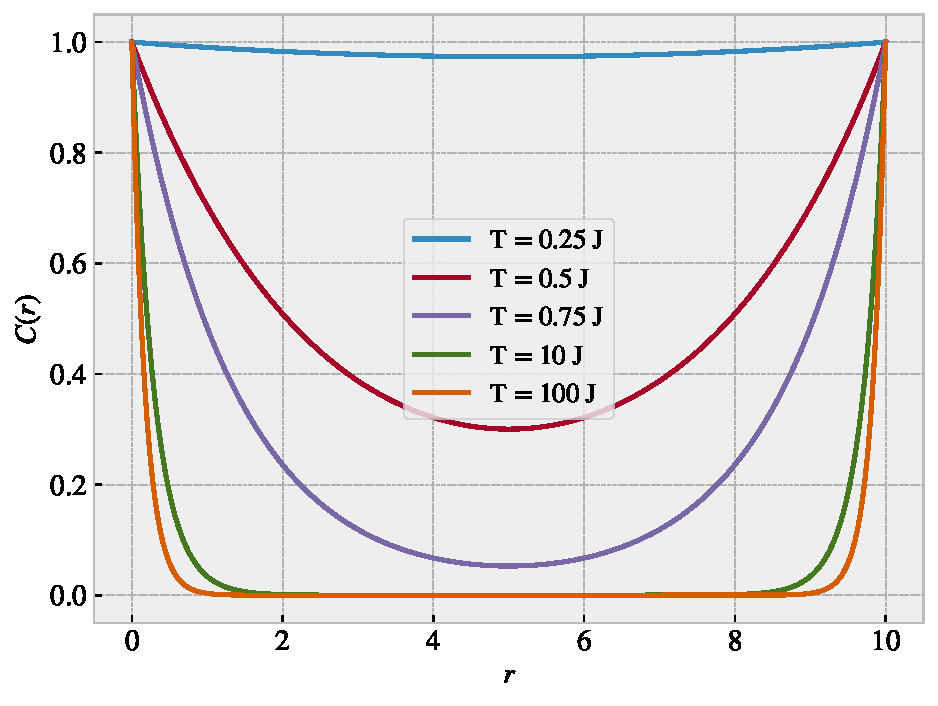
\includegraphics[width=0.6\linewidth]{figures/Cr_L10.pdf}
  \caption{Correlation function $C(r)$ from eq.~\eqref{eq:Cr_fin_L} with L = 10 for different values of $T$. }
  \label{fig:Cr_fin_L}
\end{figure}
From figure \ref{fig:Cr_fin_L} we see as expected that nearby spins is higher correlated. We remember that spins on the edge of the plot is in reality near each other due to the periodic boundary conditions. We see as expected that the spins furthest away at $r = L/2$ have the the lowest correlation value. 
\clearpage
%
%%
%%%
%%
%
\section*{Problem 2}
\subsection*{2a)}
\noindent I choose to make my own code since I wanted to make a class implementation, but I take great inspiration from that given in the exercise description. The code can be found on github: XXX. \par
In order to calculate the probability for creating bonds between sites of equal spin we use the concept of detailed balance. This corresponds to the condition
\begin{align*}
  W(\sigma)P(\sigma\to\sigma') = W(\sigma')P(\sigma'\to\sigma),
\end{align*}
where $W(\sigma) = e^{-\beta H(\sigma)}$ is the probability of being in state $\sigma$ and $P(\sigma\to\sigma')$ is the probability to transfer from state $\sigma$ to $\sigma'$. For the generalities of the Swendsen-Wang algorithm we split $P$ into two stages; Assigning bonds and flipping spins with established bonds:
\begin{align*}
  P(\sigma \to \sigma') = \underbrace{P(\sigma \to \sigma, b)}_{\text{Assign bonds}} \underbrace{\tilde{P}(\sigma, b \to\sigma',b)}_{\text{Flip spins}}
\end{align*}
While the Swendsen-Wang algorithm uses $\tilde{P} = 1/2$ the Wolff algorithm simplifies this by choosing $\tilde{P}=1$ such that the detailed balance equation reads 
\begin{align*}
  W(\sigma)P(\sigma\to\sigma, b) = W(\sigma')P(\sigma'\to\sigma', b),
\end{align*}
We denote the probability of two equal spins being bonded by $p$ where the probability of two unequal spins being bonded is always 0. The possible configurations to consider for the detailed balance equation is shown in table \ref{tab:detailed_balance}.

{\renewcommand{\arraystretch}{2}
\begin{table}[H]
  \begin{center}
  \caption{Table of possible configurations to consider for the detailed balance equations. We consider a site having spin $\bullet$ with a right neighbour having either the same spin $\bullet$ or a different spin $\circ$. Equal sites are bonded with probaility $p$ and this is marked by a connecting line --. We transfer from state $\sigma$ to $\sigma'$ by flipping the left spin, and if the spins are bonded the right spin will flip as well.}
  \begin{tabular}{|ccccc|} \hline
  \quad state $\sigma$\qquad &\qquad $W(\sigma,b)P(\sigma\to\sigma,b)$ \qquad  & Flipping spin(s) & \quad state $\sigma'$\qquad   &\qquad  $W(\sigma',b)P(\sigma'\to\sigma',b)$ \qquad \\ \hline
  $\bullet$ \ $\bullet$ & $(1-p)e^{\beta J}$ & $\Longleftrightarrow$ & $\circ$ \ $\bullet$ & $1$ \\ \hline
  $\bullet$--$\bullet$ & $pe^{\beta J}$ & $\Longleftrightarrow$ & $\circ$--$\circ$ & $pe^{\beta J}$ \\ \hline
  $\bullet$ \ $\circ$ & 1 & $\Longleftrightarrow$ & $\circ$ \ $\circ$ & $(1-p)e^{\beta J}$ \\ \hline
  \end{tabular}
  \label{tab:detailed_balance}
  \end{center}
\end{table}
{\renewcommand{\arraystretch}{1}
From table \ref{tab:detailed_balance} we only get one equation which needs to be solved for the detailed balance condition to be satsified. Solving this for $p$ we get 
\begin{align*}
  1 = (1-p)e^{\beta J} \quad \Rightarrow \quad p = 1 - e^{-\beta J}.
\end{align*}
Thus for the code we implement the probaility for equal spins to bond (pconnect) to be $p = 1 - e^{-\beta J}$. By the use of multiple bins $B$ we can calculate the sample standard deviation $s$ for a sampled quanity $x$ as
\begin{align*}
  \sigma = \sqrt{\frac{1}{B-1} \sum_{i=1}^B \Big(x_i - \Bar{x} \Big)^2}, \qquad \bar{x} = \frac{1}{B}\sum_{i=1}^B x_i,
\end{align*}
where $\bar{x}$ is the smaple mean. This serves as a way of getting error estimations on the results in the following problems.

\clearpage
\subsection*{b)}
\noindent Using the code created in a) we sample a 1D system of $L = 16$ for $T/J = 0.25$ and $T/J = 0.5$ and calculate the correlation function. This is shown in figure \ref{fig:fig2b}

\begin{figure}[H]
  \centering
  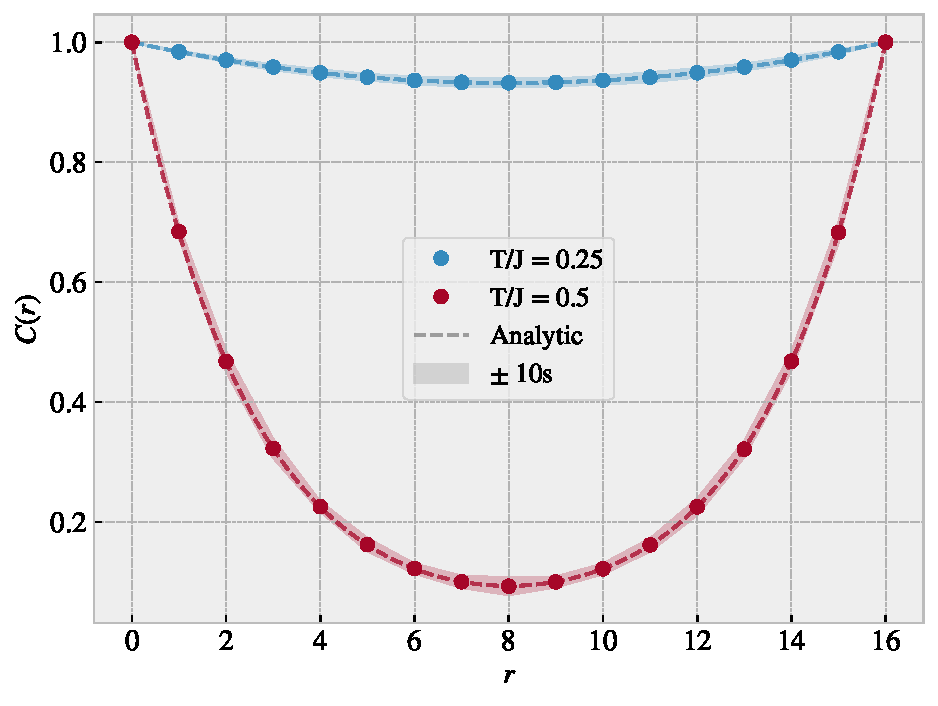
\includegraphics[width=0.6\linewidth]{figures/fig2b.pdf}
  \caption{1D chain with $L = 16$ and $10^7$ MC cycles gathered over 10 bins for each temperature sampling. The lattice was initialized with random spin direction and run for $10^6$ MC equilibriate cycles before each temperautre sampling. The shaded areas represent a $\pm 10 s$ interval for the sample standard deviation $s$. The dotted lines represent the analytic expression eq.~\eqref{eq:Cr_fin_L} found in problem 1c).}
  \label{fig:fig2b}
\end{figure}

From figure \ref{fig:fig2b} we see a very promising fit between the analytical expression and the sampling result. Considering that the error bars first show up at a $\pm 10s$ interval tells that the numerical and analytical results is in good agreement. 

\clearpage
\subsection*{c)}
\noindent We investigate the average magnetization $\langle m \rangle$ as a function of temperature for a 2D $L=16$ system. From the result in 1b) we expect this to be 0 independent of temperature. The results is shown in figure \ref{fig:fig2c}.

\begin{figure}[H]
  \centering
  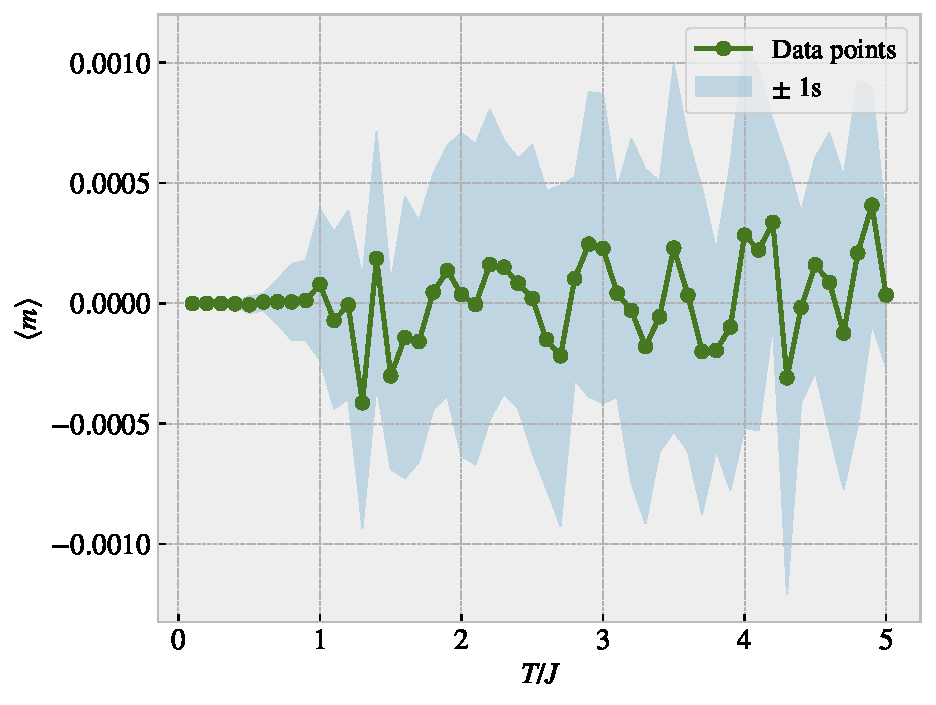
\includegraphics[width=0.6\linewidth]{figures/fig2c.pdf}
  \caption{2D lattice with $L = 16$ and $10^7$ MC cycles gathered over 10 bins for each temperature sampling in the interval $T/J \in [0.1, 10]$ with an increasing temperature step of $\Delta T/J = 0.1$. The shaded areas represent a $\pm s$ interval for the sample standard deviation $s$. The lattice was initialized with random spin direction and run for $10^6$ MC equilibriate cycles before sampling for the lowest temperature. As the temperature is increased by $\Delta T/J$ we used the last configuration from the previous sampling as the initial state for the new sampling.}
  \label{fig:fig2c}
\end{figure}

From figure \ref{fig:fig2c} we find the average magnetization to be 0 within one sample standard deviation as expected.  Even though the results gather closer around 0 for low temperature there is no indication of any trend for higher temperatures considering $\langle m \rangle$ as a function of temperature. The reason for the noise increasing with temperature is most likely due to the nature of the sampling process which seems to require even more cycles for higher temperature. 

\clearpage
\subsection*{d)}
\noindent We investigate now the average magnetization squared per site $\langle |m|^2 \rangle$ as a function of temperaure. This is shown in figure \ref{fig:fig2d}.

\begin{figure}[H]
  \centering
  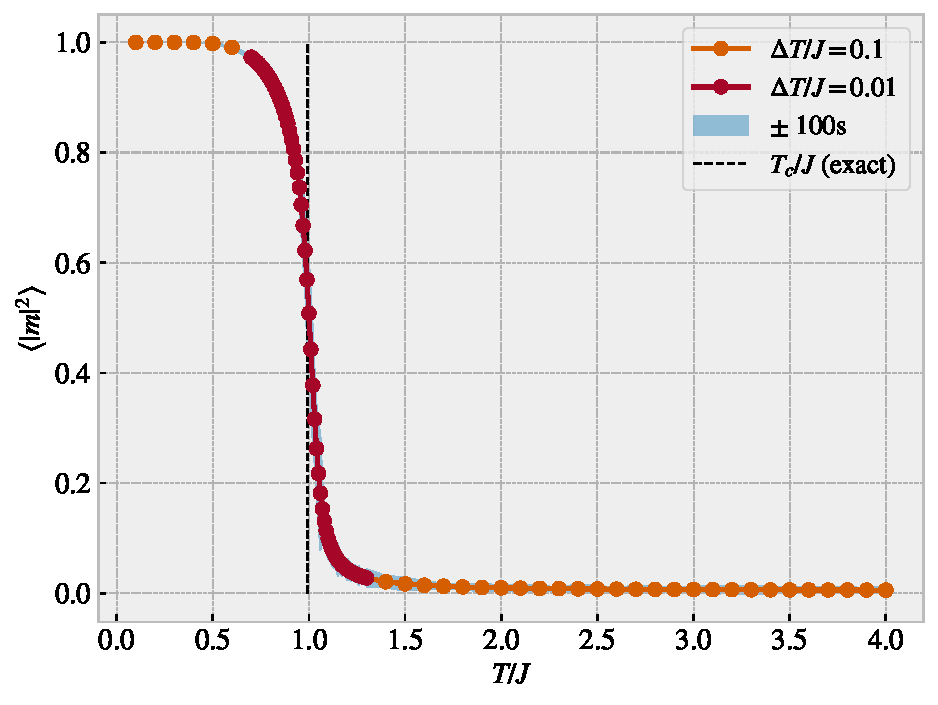
\includegraphics[width=0.6\linewidth]{figures/fig2d.pdf}
  \caption{2D lattice with $L = 16$ and $10^7$ MC cycles gathered over 10 bins for each temperature sampling in the interval $T/J \in [0.1, 10]$ with mixed temperature steps $\Delta T$ represented by the orange ($\Delta T/J = 0.1$) and red curve ($\Delta T/J = 0.01$). The two curves is produced as two independent samplings both equilibriated with $10^6$ MC equilibriate cycles and using the state from the previous temperature as initial state for the following temperatue sampling. The shaded areas represent a $\pm 100 s$ interval for the sample standard deviation $s$. The black dotted line represent the theoretical exact critical temperature $T_c/J = 1/\ln{(1 + \sqrt{3})}$.}
  \label{fig:fig2d}
\end{figure}

From figure \ref{fig:fig2d} we observe that $\langle |m|^2 \rangle$ goes from 1 (spins aligned) to 0 (spins randomely distributed) as the temperature increases past the theoretical critical temperature $T_c$. Thus the sampling captures the preference for alignment at low temperature, the preference for disorded spins at high temperature and a point of phase transistions in between which match visually well with the exact value. Considering that the error bars barely show up with a $\pm 100s$ interval this tells that these result is very certain.


\subsection*{e)}
\noindent From the theory of RG renormalization we have, for any dimensional quanity $Q$ measured in units of lattice spacing, the scaling relation
\begin{align}
  \tilde{Q}(\{k\}) = s^D \tilde{Q}(\{ks^{y_k}\}),
  \label{eq:RG}
\end{align}
where $D$ is the spatial dimensionality of $Q$, and $\tilde{Q}$ is the dimensionless version. However, when considering the dimensionless ratio
\begin{align*}
  \Gamma \equiv \frac{\langle |m|^4 \rangle}{\langle |m|^2 \rangle^2 },
\end{align*}
we have $D =0$. In addition we assume that $\Gamma = \Gamma(t, L^{-1})$ is only a function of the reduced temperatur $t \equiv (T-T_c)/T_c$, for the critical temperatur $T_c$, and inverse lattice system size $L^{-1}$. Using eq.~\ref{eq:RG} we can write
\begin{align*}
  \Gamma(t,L^{-1}) = \Gamma(ts^{y_t},L^{-1}s),
\end{align*}
where we do not include an exponent for the last variable $L^{-1}$ as it is trivial by simply being the lattice spacing. By choosing $s = L$, which is arguable the furthest we can go with the RG transformations, we get 
\begin{align*}
  \Gamma(t,L^{-1}) = \Gamma(tL^{y_t}, 1) = g(tL^{y_t}),
\end{align*}
defining the function $g(x) = \Gamma(x, 1)$. For a finite $L$ and temperatures close to the critical temperatue ($t$ close to 0) we can use a taylor expansion of $g(x)$ around $x=0$
\begin{align*}
  g(x) = g(0) + xg'(0) + \frac{1}{2}x^2 g''(0) + \cdots,
\end{align*}  
which gives 
\begin{align*}
  \Gamma(t,L^{-1}) = g(0) + tL^{y_t}g'(0) + \frac{1}{2}(tL^{y_t})^2g''(0) + \cdots.
\end{align*}
Thus for a finite $L$ as $t \to 0$ the series will simply become
\begin{align}
 \left. \Gamma(t,L^{-1}) \right|_{t=0} = g(0).
 \label{eq:intersec}
\end{align}
This shows that all curves of $\Gamma$ vs. $T/J$ should cross at the phase transistion temperatue in $(T_c, g(0))$ independent of system size $L$.


\subsection*{f)}
\noindent Testing the statement from 2e) we sample a 2D lattice with size $L = \{8, 16, 32\}$ and plot $\Gamma$ vs. $T/J$ looking for intersection points. 
The result is showbn in figure \ref{fig:fig2f}.

\begin{figure}[H]
  \centering
  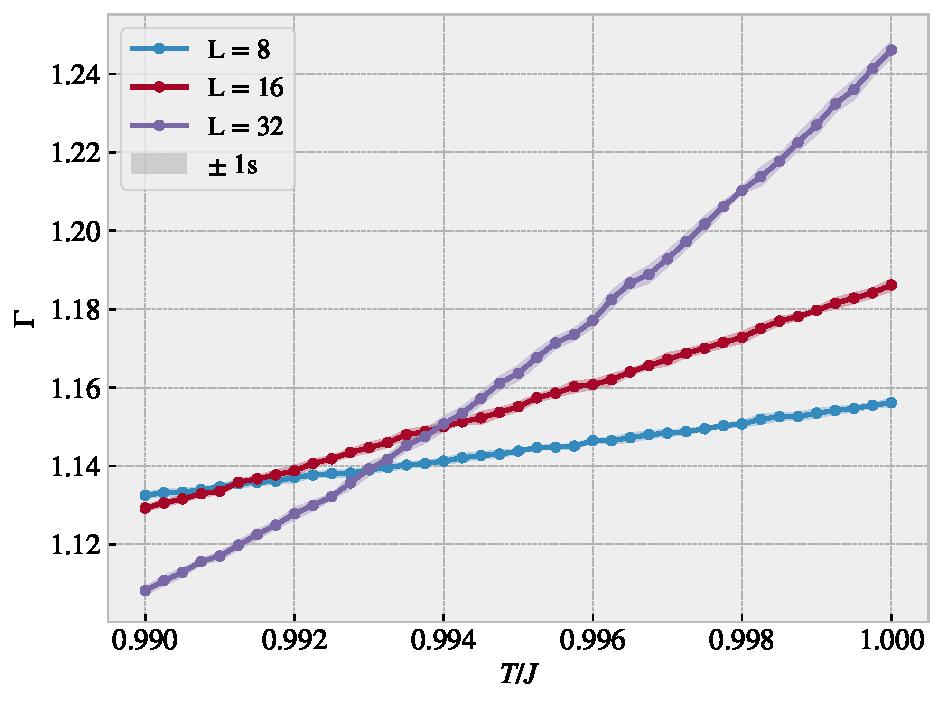
\includegraphics[width=0.6\linewidth]{figures/fig2f.pdf}
  \caption{$\Gamma$ vs. $T/J$ for 2D lattices of size $L = \{8,16,32\}$ with $10^7$ MC cycles gathered over 10 bins for each temperature sampling in the interval $T/J \in [0.99, 1]$ with an increasing temperature step of $\Delta T/J = 0.00025$. The shaded areas represents a $\pm 1 s$ interval for the sample standard deviation $s$. The lattice was initialized with random spin direction and run for $10^6$ MC equilibriate cycles before sampling for the lowest temperature. As the temperature is increased by $\Delta T/J$ we used the last configuration from the previous sampling as the initial state for the new sampling.}
  \label{fig:fig2f}
\end{figure}

From figure \ref{fig:fig2f} we do not get a single unique intersection point as an estmate for $T_c$, as suggested by eq.~\eqref{eq:intersec}, but rather two candidates. That is the intersection between the lines  $l_{L=8}$ and $l_{L=16}$, and $l_{L=16}$ and $l_{L=32}$ respectively
\begin{align*}
  l_{L=8} \cap l_{L=16} &= 0.9912 \pm \num{9e-04}, \\
  l_{L=16} \cap l_{L=32} &= 0.9939 \pm \num{4e-04}, \\
  \text{Average} &=  0.9926 \pm \num{6e-04}.
\end{align*}
When comparing to the theoretical exact result $T/J = 1/\ln{(1 + \sqrt{3})} \approx 0.9950$ we see that both intersection points falls slightly short of the exact result. However, we notice that the estimate seems to get better for higher value of $L$. \par 
A possible explanation for this, is that the assumption $\Gamma = \Gamma(t, L^{-1})$ might not be valid. Let us now assume that $\Gamma$ is also a function of some variable $k$ for which there exist an attractive fix point with $y_k < 0$. That is, $k$ is an irrelevant coupling. Including this into the RG equation eq.~\ref{eq:RG} we get 
\begin{align*}
  \Gamma(t,L^{-1}, k) = \Gamma(ts^{y_t},L^{-1}s, ks^{y_k}), \qquad y_t > 0, \ y_k < 0
\end{align*}
By choosing $s = L$ we now get a different expression
\begin{align*}
  \Gamma(t,L^{-1}, k) = \Gamma(tL^{y_t}, 1, kL^{y_k}) = h(tL^{y_t}, kL^{y_k}),
\end{align*}
where we defined the new function $h(x, y) = \Gamma(x, 1, y)$. We are still interested in the behaviour around the critical temperatur and thus it is still reasonable to use a taylor expansion for $x = 0$, but as we choose a general point $b$ for the expansion of $y$ we get
\begin{align*}
  h(x,y) &= h(0,b) + x\frac{\partial h(0,b)}{\partial x} + (y-b)\frac{\partial h(0,b)}{\partial y} + \frac{1}{2!}\Big[x^2\frac{\partial ^2h(0,b)}{\partial x^2} + 2x(y-b) \frac{\partial ^2h(0,b)}{\partial x\partial y} + (y-b)^2\frac{\partial ^2h(0,b)}{\partial y^2} \Big] + \hdots \\
  h(tL^{y_t},  kL^{y_k}) &= h(0,b) + tL^{y_t}\frac{\partial h(0,b)}{\partial x} + (kL^{y_k}-b)\frac{\partial h(0,b)}{\partial y} \\
  &\qquad \qquad \qquad \qquad \qquad \ \ + \frac{1}{2!}\Big[(tL^{y_t})^2\frac{\partial ^2h(0,b)}{\partial x^2} + 2tL^{y_t}(kL^{y_k}-b) \frac{\partial ^2h(0,b)}{\partial x\partial y} + (kL^{y_k}-b)^2\frac{\partial ^2h(0,b)}{\partial y^2} \Big] + \hdots
\end{align*}

For $t\to 0$ we are left with some $L$ dependence
\begin{align*}
  \left. \Gamma(t, L^{-1},k) \right|_{t=0} = h(0,b) + (kL^{y_k}-b)\frac{\partial h(0,b)}{\partial y} + \frac{1}{2!}(kL^{y_k}-b)^2\frac{\partial ^2h(0,b)}{\partial y^2} + \hdots 
\end{align*}
Even if we assume $k$ to be small at the critical temperatue such that we can choose $b = 0$ we are left with $L$ dependence
\begin{align*}
  \left. \Gamma(t, L^{-1},k) \right|_{t=0, b = 0} = h(0,0) + kL^{y_k}\frac{\partial h(0,0)}{\partial y} + \frac{1}{2!}(kL^{y_k})^2\frac{\partial ^2h(0,0)}{\partial y^2} + \hdots
\end{align*}
However, as $y_k < 0$ this added contribution $\propto kL^{y_k}$ will vanish for increasing $L$, where the speed of this depends on the absolute value of $y_k$. If the absolute value of $y_k$ is small one will need a bigger $L$ for the contribution to vanish in practice. This explains why the intersections in figure \ref{fig:fig2f} gives the more accurate result for the biggest system sizes. If we were to sample with bigger system size, we would expect the intersection point to approach $T_c$ even closer.


%%%%%%%%%%%%%%%%%%%%%%%%%%%%%%%%%%%%%%%%%%%%%%%%%%%%%%%%%%% 

\begin{thebibliography}{}
  \bibitem{Svendsen} Svendsen, Robert H., An introduction to Statistical Mechanics and Thermodynamics, Second edition 2020.
\end{thebibliography}
\clearpage

\appendix
\section{Linear algebra for the transfer matrix T}
\noindent In problem 1 we work with the transfer matrix
\begin{align*}
  T = \begin{pmatrix}
        e^{\beta J} & 1 & 1 \\
        1 & e^{\beta J} & 1 \\
        1 & 1 & e^{\beta J}
      \end{pmatrix}.
\end{align*}
In order to ease the calculations we needed the eigenvalues, eigenvectors and the diagonalization of $T$. These calculations is carried out in the following subsections.
%
%%
%
\subsection{Eigenvalues}\label{sec:T_eigval}
\noindent We get the characteristic equation 
\begin{align*}
  \det{(T - \lambda \mathbb{I} )} 
  = \begin{vmatrix}
    e^{\beta J} -\lambda & 1 & 1 \\
    1 & e^{\beta J} -\lambda & 1 \\
    1 & 1 & e^{\beta J} -\lambda
  \end{vmatrix} = 0.
\end{align*}
We introduce $x = e^{\beta J} -\lambda$ and find
\begin{align*}
  \det{(T - \lambda \mathbb{I} )} 
  = \begin{vmatrix}
    x & 1 & 1 \\
    1 & x & 1 \\
    1 & 1 & x
  \end{vmatrix}
  &= x \begin{vmatrix} 
            x & 1 \\ 
            1 & x  
        \end{vmatrix}
      - \begin{vmatrix} 
        1 & 1 \\ 
        1 & x   
        \end{vmatrix} 
      + \begin{vmatrix} 
        1 & x \\ 
        1 & 1   
        \end{vmatrix} = (x^3 - x) - (x - 1) + (1 - x) = x^3 - 3x + 2 = 0.
\end{align*}
We see that $x = 1$ is a root and thus we can do polynomial division
\begin{align*}
  {\polylongdiv{x^3 - 3x + 2}{x-1}},
\end{align*}
which yields the factorized expression 
\begin{align*}
  (x^2 + x -2)(x-1) = 0.
\end{align*}
Solving for the first quadratic factor we get 
\begin{align*}
  x = \frac{-1 \pm \sqrt{1 + 8}}{2} = 1 \vee -2.
\end{align*}
Changing back from $x$ to $\lambda$ using $\lambda = e^{\beta J}-x$ we arrive at the eigenvalues
\begin{align*}
  \lambda_1 = \lambda_2 = e^{\beta J} - 1, \qquad \lambda_2 = e^{\beta J} + 2
\end{align*}
%
%%
%¨
\subsection{Eigenvectors}\label{sec:T_eigvec}
The eigenvectors must satisfy 
\begin{align*}
  (T - \lambda \mathbb{I} ) = \vec{0}.
\end{align*}
The first two eigenvectors $v_1$ and $v_2$ corresponding to $\lambda_1$ and $\lambda_2$ is on the form
\begin{align*}
  \begin{pmatrix}
    1 & 1 & 1 \\
    1 & 1 & 1 \\
    1 & 1 & 1
  \end{pmatrix} 
  \sim
  \begin{pmatrix}
    1 & 1 & 1 \\
    0 & 0 & 0 \\
    0 & 0 & 0
  \end{pmatrix} 
  = \vec{0} \quad 
  \Rightarrow \quad 
  x + y + z = 0.
\end{align*} 
Thus two linearly indpendent eigenvectors for $v_1$ and $v_2$ is 
\begin{align*}
  v_1 = \begin{pmatrix} -1 \\ 1 \\ 0 \end{pmatrix}, \qquad 
  v_1 = \begin{pmatrix} -1 \\ 0 \\ 1 \end{pmatrix}.
\end{align*}
The third eigenvector $v_3$ is on the form
\begin{align*}
  \begin{pmatrix}
    -2 & 1 & 1 \\
    1 & -2 & 1 \\
    1 & 1 & -2
  \end{pmatrix} 
  \sim
  \begin{pmatrix}
    1 & -2 & 1 \\
    0 & 3 & -3 \\
    0 & 3 & -3
  \end{pmatrix} 
  \sim
  \begin{pmatrix}
    1 & 0 & -1 \\
    0 & 1 & -1 \\
    0 & 0 & 0
  \end{pmatrix} 
  = \vec{0} \quad
  \Rightarrow \quad 
  x = y = z
\end{align*}
One possible eigenvector is thus 
\begin{align*}
  v_3 = \begin{pmatrix} 1 \\ 1 \\ 1 \end{pmatrix}.
\end{align*}

\subsection{Diagonalization of T}\label{sec:T_diag}
\noindent We can diagonalize $T$ as $T=PDP^{-1}$ where $D$ is a diagonal matrix containing the eigenvalues of $T$, and $P$ is invertible and created such that the column vectors form a basis consisting of eigenvectors of $T$. Given the eigenvalues and eigenvectors found in \ref{sec:T_eigvec} and \ref{sec:T_eigval} respectively we have 
\begin{align*}
  D =  \begin{pmatrix}
       e^{\beta J} - 1 & 0 & 0 \\
       0 & e^{\beta J} - 1 & 0 \\
       0 & 0 & e^{\beta J} + 2
       \end{pmatrix}, 
       \qquad 
  P = \begin{pmatrix}
      -1 & -1 & 1 \\
       1 & 0 & 1 \\
      0 & 1 & 1
      \end{pmatrix}  
\end{align*}
We find the invers of $P$.
\begin{align*}
    \left(\begin{array}{ccc|ccc}
    -1 & -1 & 1  & 1 & 0 & 0 \\
    1  & 0  & 1  & 0 & 1 & 0 \\
    0  & 1  & 0  & 0 & 0 & 1 \\
    \end{array}\right)
    \sim 
    \left(\begin{array}{ccc|ccc}
    1 & 1  & -1 & -1 & 0 & 0 \\
    0 & -1 & 2  & 1  & 1 & 0 \\
    0 & 1  & 1  & 0  & 0 & 1 \\
    \end{array}\right)
    \sim   
    \left(\begin{array}{ccc|ccc}
    1 & 0  & 1 & 0 & 1 & 0 \\
    0 & 1 & -2  & -1  & -1 & 0 \\
    0 & 0  & 3  & 1  & 1 & 1 \\
    \end{array}\right)
    \sim   
    \left(\begin{array}{ccc|ccc}
    1 & 0 & 0  & -1/3 & 2/3 & -1/3 \\
    0 & 1 & 0  & -1/3  & -1/3 & 2/3 \\
    0 & 0 & 1  & 1/3  & 1/3 & 1/3 \\
    \end{array}\right).
\end{align*}
This gives 
\begin{align*}
  P^{-1} =  \frac{1}{3}
  \begin{pmatrix}
    -1 & 2 & -1 \\
    -1 & -1 & 2 \\
    1 & 1 & 1
  \end{pmatrix}  
\end{align*}
Combining the above results we get the diagonalization as follows.
\begin{align*}
  T = \begin{pmatrix}
     -1 & -1 & 1 \\
      1 & 0 & 1 \\
      0 & 1 & 1
    \end{pmatrix}  
    \begin{pmatrix}
      e^{\beta J} - 1 & 0 & 0 \\
       0 & e^{\beta J} - 1 & 0 \\
       0 & 0 & e^{\beta J} + 2
     \end{pmatrix} 
     \frac{1}{3} 
     \begin{pmatrix}
      -1 & 2 & -1 \\
       -1 & -1 & 2 \\
       1 & 1 & 1
     \end{pmatrix}.  
\end{align*}
In addition we will need the expression for $T^l$ where $l$ is some positive integer exponent. Using the diagonalization this can be calcuolated as
\begin{align*}
  T^l = \underbrace{(PDP^{-1})(PDP^{-1})\cdots(PDP^{-1})}_{l} = PD^lP^{-1}.
\end{align*}
Since $D^l$ is trivial to calculate for a diagonal matrix we get
{\renewcommand{\arraystretch}{1.5}
\begin{align*}
  T^l &= 
  \begin{pmatrix}
    -1 & -1 & 1 \\
     1 & 0 & 1 \\
     0 & 1 & 1
   \end{pmatrix}  
   \begin{pmatrix}
    (e^{\beta J} - 1)^l & 0 & 0 \\
    0 & (e^{\beta J} - 1)^l & 0 \\
    0 & 0 & (e^{\beta J} + 2)^l
    \end{pmatrix} 
    \frac{1}{3} 
    \begin{pmatrix}
    -1 & 2 & -1 \\
    -1 & -1 & 2 \\
    1 & 1 & 1
    \end{pmatrix} \\
    &= 
  \begin{pmatrix}
    -(e^{\beta J} - 1)^l & -(e^{\beta J} - 1)^l & (e^{\beta J} + 2)^l \\
    \ \ (e^{\beta J} - 1)^l & 0 & (e^{\beta J} + 2)^l \\
     0 & \ \ (e^{\beta J} - 1)^l & (e^{\beta J} + 2)^l
   \end{pmatrix}  
    \frac{1}{3} 
    \begin{pmatrix}
    -1 & 2 & -1 \\
    -1 & -1 & 2 \\
    1 & 1 & 1
    \end{pmatrix} \\
    &= 
    \frac{1}{3}
    \begin{pmatrix}
      2a + b & -a + b & -a + b \\
      -a + b & 2a + b & -a + b \\
      -a + b & -a + b & 2a + b
    \end{pmatrix}, \qquad 
    a =  (e^{\beta J} - 1)^l, \ b = (e^{\beta J} + 2)^l
\end{align*}
It turs out that the resulting matrix only have to distinct values, one for the diagonal elements and one for the off-diagonal elements
\begin{align*}
  T^l_{i,j} = 
  \begin{cases}
    \frac{1}{3}\Big[ 2(e^{\beta J} - 1)^l + (e^{\beta J} + 2)^l\Big], & i = j \\[8 pt]
    \frac{1}{3}\Big[ -(e^{\beta J} - 1)^l + (e^{\beta J} + 2)^l \Big], & i \neq j \ .
  \end{cases}
\end{align*}
Notice that for $l = L$ we get $T^L_{i,i} = Z/3$.


\end{document}
